\documentclass{beamer}
\usetheme{Madrid}
\usecolortheme{default}
\usepackage{graphicx}
\usepackage{hyperref}
\usepackage{tikz}
\usepackage{listings}
\usepackage{xcolor}

\title{Multimedia Technology Fundamentals}
\subtitle{A Comprehensive Guide}
\author{MMT Class}
\date{\today}

\begin{document}

\frame{\titlepage}

\begin{frame}{Table of Contents}
\tableofcontents
\end{frame}

\section{Multimedia Basics}

\begin{frame}{What is Multimedia?}
\begin{itemize}
\item \textbf{Definition:} Integration of multiple forms of media
\item Text, Audio, Video, Graphics, Animation
\item Interactive and non-linear content delivery
\item \textbf{Real Example:} Netflix combines video, audio, subtitles, interactive menus
\end{itemize}
\begin{block}{Key Characteristics}
\begin{itemize}
\item Digital representation
\item Computer-controlled
\item Interactive user experience
\end{itemize}
\end{block}
\end{frame}

\begin{frame}{Multimedia Applications}
\begin{columns}
\column{0.5\textwidth}
\textbf{Entertainment:}
\begin{itemize}
\item Gaming (PlayStation, Xbox)
\item Streaming (YouTube, Spotify)
\item Virtual Reality
\end{itemize}
\vspace{0.3cm}
\centering
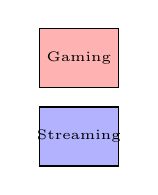
\begin{tikzpicture}[scale=0.5]
\draw[fill=red!30] (0,0) rectangle (2,1.5);
\node at (1,0.75) {\tiny Gaming};
\draw[fill=blue!30] (0,-2) rectangle (2,-0.5);
\node at (1,-1.25) {\tiny Streaming};
\end{tikzpicture}
\column{0.5\textwidth}
\textbf{Professional:}
\begin{itemize}
\item E-learning platforms
\item Medical imaging
\item Digital marketing
\end{itemize}
\vspace{0.3cm}
\centering
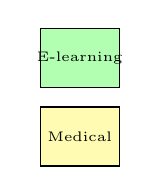
\begin{tikzpicture}[scale=0.5]
\draw[fill=green!30] (0,0) rectangle (2,1.5);
\node at (1,0.75) {\tiny E-learning};
\draw[fill=yellow!30] (0,-2) rectangle (2,-0.5);
\node at (1,-1.25) {\tiny Medical};
\end{tikzpicture}
\end{columns}
\end{frame}

\begin{frame}{Hypermedia Explained}
\begin{itemize}
\item \textbf{Extension of hypertext} with multimedia elements
\item Non-linear navigation through content
\item Links connect text, images, audio, video
\item \textbf{Example:} Wikipedia articles with embedded videos, images, and cross-references
\end{itemize}
\begin{alertblock}{Hypermedia vs Multimedia}
Hypermedia = Multimedia + Hyperlinks + Non-linear Navigation
\end{alertblock}
\end{frame}

\begin{frame}{World Wide Web (WWW)}
\begin{columns}
\column{0.55\textwidth}
\begin{itemize}
\item Created by Tim Berners-Lee (1989)
\item Information system on Internet
\item Documents via hyperlinks
\item Accessed through browsers
\end{itemize}
\begin{block}{WWW Components}
\begin{itemize}
\item \textbf{HTTP/HTTPS:} Protocol
\item \textbf{URL:} Resource ID
\item \textbf{HTML:} Markup language
\end{itemize}
\end{block}
\column{0.45\textwidth}
\centering
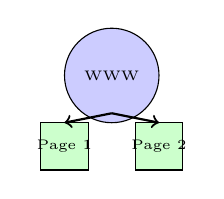
\begin{tikzpicture}[scale=0.6]
\draw[fill=blue!20] (0,0) circle (1);
\node at (0,0) {\tiny WWW};
\draw[fill=green!20] (-1.5,-2) rectangle (-0.5,-1);
\node at (-1,-1.5) {\tiny Page 1};
\draw[fill=green!20] (0.5,-2) rectangle (1.5,-1);
\node at (1,-1.5) {\tiny Page 2};
\draw[->,thick] (0,-0.8) -- (-1,-1);
\draw[->,thick] (0,-0.8) -- (1,-1);
\end{tikzpicture}
\end{columns}
\end{frame}

\begin{frame}{Internet Architecture}
\begin{columns}
\column{0.55\textwidth}
\begin{itemize}
\item Global network of computers
\item \textbf{Client-Server Model}
\item \textbf{Protocols:} TCP/IP, HTTP
\end{itemize}
\textbf{Accessing Amazon.com:}
\begin{enumerate}
\item DNS resolves domain
\item TCP connection
\item HTTP request sent
\item Server responds
\end{enumerate}
\column{0.45\textwidth}
\centering
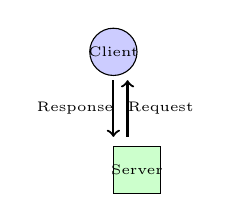
\begin{tikzpicture}[scale=0.6]
\draw[fill=blue!20] (0,3) circle (0.5);
\node at (0,3) {\tiny Client};
\draw[fill=green!20] (0,0) rectangle (1,1);
\node at (0.5,0.5) {\tiny Server};
\draw[->,thick] (0,2.4) -- (0,1.2);
\node[right] at (0.1,1.8) {\tiny Request};
\draw[->,thick] (0.3,1.2) -- (0.3,2.4);
\node[left] at (0.2,1.8) {\tiny Response};
\end{tikzpicture}
\end{columns}
\end{frame}

\begin{frame}{Internet vs WWW}
\begin{center}
\begin{tabular}{|p{5cm}|p{5cm}|}
\hline
\textbf{Internet} & \textbf{WWW} \\
\hline
Hardware infrastructure & Software service \\
Network of networks & Information system \\
Includes email, FTP, VoIP & Web pages and websites \\
Exists since 1960s & Created in 1989 \\
\hline
\end{tabular}
\end{center}
\end{frame}

\begin{frame}{Multimedia Software Categories}
\begin{enumerate}
\item \textbf{Content Creation:} Adobe Creative Suite, Blender
\item \textbf{Editing Tools:} Premiere Pro, Audacity, GIMP
\item \textbf{Authoring Tools:} Adobe Animate, Unity
\item \textbf{Playback Software:} VLC, Windows Media Player
\item \textbf{Compression Tools:} HandBrake, FFmpeg
\end{enumerate}
\end{frame}

\begin{frame}{Editing Tools Overview}
\begin{block}{Image Editing}
\textbf{Adobe Photoshop:} Professional raster graphics editor\\
\textbf{GIMP:} Free alternative for image manipulation\\
\textbf{Use Case:} Photo retouching, color correction, compositing
\end{block}
\begin{block}{Video Editing}
\textbf{Adobe Premiere Pro:} Industry-standard video editor\\
\textbf{DaVinci Resolve:} Professional color grading\\
\textbf{Use Case:} YouTube content creation, film production
\end{block}
\end{frame}

\begin{frame}{Audio Editing Tools}
\begin{itemize}
\item \textbf{Audacity:} Free, open-source audio editor
\item \textbf{Adobe Audition:} Professional audio workstation
\item \textbf{Pro Tools:} Industry standard for music production
\end{itemize}
\begin{exampleblock}{Real Scenario: Podcast Production}
\begin{enumerate}
\item Record audio with microphone
\item Import into Audacity
\item Remove background noise
\item Normalize audio levels
\item Export as MP3 for distribution
\end{enumerate}
\end{exampleblock}
\end{frame}

\begin{frame}{Authoring Tools}
\begin{itemize}
\item Software for creating multimedia presentations
\item Combine text, graphics, audio, video, animation
\item \textbf{Examples:}
\begin{itemize}
\item Adobe Animate (Flash successor)
\item Unity (Game development)
\item Articulate Storyline (E-learning)
\item H5P (Interactive HTML5 content)
\end{itemize}
\end{itemize}
\end{frame}

\begin{frame}{Authoring Paradigms}
\begin{enumerate}
\item \textbf{Card/Page-Based:} PowerPoint, Keynote
\item \textbf{Timeline-Based:} Adobe Animate, After Effects
\item \textbf{Icon/Flow-Based:} Authorware (legacy)
\item \textbf{Programming-Based:} Unity, Unreal Engine
\end{enumerate}
\begin{block}{Choosing the Right Tool}
Consider: Project complexity, interactivity needs, target platform, budget
\end{block}
\end{frame}

\section{Graphics and Image Data Representation}

\begin{frame}{Graphics Data Types}
\begin{columns}
\column{0.5\textwidth}
\textbf{Raster Graphics:}
\begin{itemize}
\item Pixel-based images
\item Resolution-dependent
\item Photos, digital paintings
\item Examples: JPEG, PNG, BMP
\end{itemize}
\column{0.5\textwidth}
\textbf{Vector Graphics:}
\begin{itemize}
\item Mathematical equations
\item Resolution-independent
\item Logos, illustrations
\item Examples: SVG, AI, EPS
\end{itemize}
\end{columns}
\end{frame}

\begin{frame}{Raster vs Vector: Visual Comparison}
\begin{center}
\includegraphics[width=0.7\textwidth]{images/raster_vector.png}
\end{center}
\vspace{0.2cm}
\textbf{Key:} Raster loses quality when scaled; Vector maintains quality
\end{frame}

\begin{frame}{Image Resolution and Quality}
\begin{columns}
\column{0.6\textwidth}
\begin{itemize}
\item \textbf{Resolution:} Pixels (width × height)
\item \textbf{DPI/PPI:} Dots/Pixels per inch
\item \textbf{Common Resolutions:}
\begin{itemize}
\item HD: 1920×1080 (2.1 MP)
\item 4K: 3840×2160 (8.3 MP)
\item 8K: 7680×4320 (33.2 MP)
\end{itemize}
\end{itemize}
\column{0.4\textwidth}
\centering
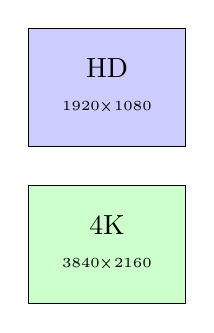
\begin{tikzpicture}
\draw[fill=blue!20] (0,0) rectangle (2,1.5);
\node at (1,1) {HD};
\node at (1,0.5) {\tiny 1920×1080};
\draw[fill=green!20] (0,-2) rectangle (2,-0.5);
\node at (1,-1) {4K};
\node at (1,-1.5) {\tiny 3840×2160};
\end{tikzpicture}
\end{columns}
\end{frame}

\begin{frame}{Popular Image File Formats}
\begin{center}
\begin{tabular}{|l|l|l|l|}
\hline
\textbf{Format} & \textbf{Type} & \textbf{Compression} & \textbf{Use Case} \\
\hline
JPEG & Raster & Lossy & Photos \\
PNG & Raster & Lossless & Web graphics \\
GIF & Raster & Lossless & Animations \\
BMP & Raster & None & Raw images \\
SVG & Vector & N/A & Logos, icons \\
TIFF & Raster & Both & Professional \\
\hline
\end{tabular}
\end{center}
\end{frame}

\begin{frame}{JPEG Format Deep Dive}
\begin{itemize}
\item \textbf{Full Name:} Joint Photographic Experts Group
\item \textbf{Compression:} Lossy (DCT-based)
\item \textbf{Color Support:} 24-bit (16.7 million colors)
\item \textbf{Advantages:} Small file size, universal support
\item \textbf{Disadvantages:} Quality loss, no transparency
\end{itemize}
\begin{block}{Real Scenario}
Digital camera: 5MB RAW → 500KB JPEG for social media
\end{block}
\end{frame}

\begin{frame}{PNG Format}
\begin{itemize}
\item \textbf{Full Name:} Portable Network Graphics
\item \textbf{Compression:} Lossless (DEFLATE algorithm)
\item \textbf{Features:}
\begin{itemize}
\item Transparency support (alpha channel)
\item Better for text and line art
\item No quality loss on re-saving
\end{itemize}
\item \textbf{Use Case:} Website logos, UI elements, screenshots
\end{itemize}
\end{frame}

\begin{frame}{GIF Format}
\begin{itemize}
\item \textbf{Full Name:} Graphics Interchange Format
\item \textbf{Color Limit:} 256 colors (8-bit)
\item \textbf{Features:} Animation support, transparency
\item \textbf{Modern Alternative:} WebP, APNG
\end{itemize}
\begin{exampleblock}{Real Example}
Twitter/X reaction GIFs, animated emojis, simple animations
\end{exampleblock}
\end{frame}

\begin{frame}{SVG Format}
\begin{itemize}
\item \textbf{Full Name:} Scalable Vector Graphics
\item \textbf{Based on:} XML text format
\item \textbf{Advantages:}
\begin{itemize}
\item Infinite scalability
\item Small file size for simple graphics
\item Editable with text editors
\item CSS and JavaScript compatible
\end{itemize}
\item \textbf{Use Case:} Responsive web design, icons, logos
\end{itemize}
\end{frame}

\begin{frame}{WebP and Modern Formats}
\begin{itemize}
\item \textbf{WebP:} Google's modern image format
\item Supports both lossy and lossless compression
\item 25-35\% smaller than JPEG/PNG
\item Transparency and animation support
\item \textbf{AVIF:} Next-gen format, even better compression
\end{itemize}
\begin{block}{Adoption}
Used by Google, Facebook, Netflix for faster web performance
\end{block}
\end{frame}

\section{Color in Image}

\begin{frame}{Color Science Fundamentals}
\begin{itemize}
\item \textbf{Light:} Electromagnetic radiation (380-750 nm)
\item \textbf{Human Eye:} Three types of cone cells
\begin{itemize}
\item S-cones: Short wavelength (blue)
\item M-cones: Medium wavelength (green)
\item L-cones: Long wavelength (red)
\end{itemize}
\item \textbf{Color Perception:} Brain interprets signals from cones
\end{itemize}
\end{frame}

\begin{frame}{Additive vs Subtractive Color}
\begin{columns}
\column{0.5\textwidth}
\textbf{Additive (RGB):}
\begin{itemize}
\item Light-based
\item Red + Green + Blue
\item Used in displays
\item More light = brighter
\end{itemize}
\centering
\includegraphics[width=0.6\textwidth]{images/rgb.png}
\column{0.5\textwidth}
\textbf{Subtractive (CMYK):}
\begin{itemize}
\item Pigment-based
\item Cyan + Magenta + Yellow
\item Used in printing
\item More ink = darker
\end{itemize}
\centering
\includegraphics[width=0.6\textwidth]{images/cmyk.png}
\end{columns}
\end{frame}

\begin{frame}{RGB Color Model}
\begin{columns}
\column{0.55\textwidth}
\begin{itemize}
\item \textbf{Primary:} Red, Green, Blue
\item \textbf{Bit Depth:} 8 bits/channel
\item \textbf{Range:} 0-255 (16.7M colors)
\item \textbf{Examples:}
\begin{itemize}
\item Red: (255, 0, 0)
\item White: (255, 255, 255)
\item Black: (0, 0, 0)
\item Purple: (128, 0, 128)
\end{itemize}
\end{itemize}
\column{0.45\textwidth}
\centering
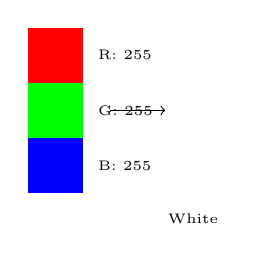
\begin{tikzpicture}[scale=0.7]
\fill[red] (0,2) rectangle (1,3);
\node[right] at (1.1,2.5) {\tiny R: 255};
\fill[green] (0,1) rectangle (1,2);
\node[right] at (1.1,1.5) {\tiny G: 255};
\fill[blue] (0,0) rectangle (1,1);
\node[right] at (1.1,0.5) {\tiny B: 255};
\draw[->] (1.5,1.5) -- (2.5,1.5);
\fill[white] (2.5,0.5) rectangle (3.5,2.5);
\node[below] at (3,-0.2) {\tiny White};
\end{tikzpicture}
\end{columns}
\end{frame}

\begin{frame}{CMYK Color Model}
\begin{itemize}
\item \textbf{Components:} Cyan, Magenta, Yellow, Key (Black)
\item \textbf{Values:} 0-100\% for each channel
\item \textbf{Why K (Black)?:} Pure CMY mix creates muddy brown
\item \textbf{Use Case:} Professional printing, magazines, brochures
\end{itemize}
\begin{alertblock}{Important}
Always convert RGB to CMYK before printing to avoid color shifts
\end{alertblock}
\end{frame}

\begin{frame}{HSV/HSB Color Model}
\begin{columns}
\column{0.5\textwidth}
\begin{itemize}
\item \textbf{H:} Hue (0-360°)
\item \textbf{S:} Saturation (0-100\%)
\item \textbf{V/B:} Value/Brightness
\item More intuitive for humans
\item Used in color pickers
\end{itemize}
\column{0.5\textwidth}
\centering
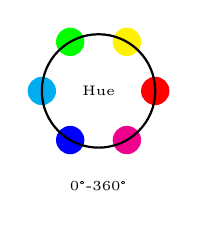
\begin{tikzpicture}[scale=0.6]
\foreach \angle/\col in {0/red, 60/yellow, 120/green, 180/cyan, 240/blue, 300/magenta}
  \fill[\col] (\angle:1.2) circle (0.3);
\draw[thick] (0,0) circle (1.2);
\node at (0,0) {\tiny Hue};
\node at (0,-2) {\tiny 0°-360°};
\end{tikzpicture}
\end{columns}
\end{frame}

\begin{frame}{HSL Color Model}
\begin{itemize}
\item \textbf{H:} Hue (0-360°)
\item \textbf{S:} Saturation (0-100\%)
\item \textbf{L:} Lightness (0-100\%)
\item \textbf{Difference from HSV:} Lightness calculation
\item \textbf{Use Case:} CSS color definitions in web development
\end{itemize}
\begin{exampleblock}{CSS Example}
\texttt{color: hsl(120, 100\%, 50\%);} // Pure green
\end{exampleblock}
\end{frame}

\begin{frame}{YUV/YCbCr Color Model}
\begin{itemize}
\item \textbf{Y:} Luma (brightness)
\item \textbf{U/Cb:} Blue-difference chroma
\item \textbf{V/Cr:} Red-difference chroma
\item \textbf{Advantage:} Separates brightness from color
\item \textbf{Use Case:} Video compression (JPEG, MPEG, H.264)
\end{itemize}
\begin{block}{Why YUV?}
Human eye more sensitive to brightness than color → Can compress chroma more
\end{block}
\end{frame}

\begin{frame}{Color Depth and Bit Depth}
\begin{itemize}
\item \textbf{1-bit:} 2 colors (black \& white)
\item \textbf{8-bit:} 256 colors (GIF)
\item \textbf{24-bit:} 16.7M colors (True Color)
\item \textbf{32-bit:} 24-bit + 8-bit alpha (transparency)
\item \textbf{48-bit:} Professional photography (16-bit per channel)
\end{itemize}
\begin{exampleblock}{File Size Impact}
1920×1080 image: 24-bit = 6.2MB, 8-bit = 2.1MB (uncompressed)
\end{exampleblock}
\end{frame}

\begin{frame}{Color Spaces and Gamut}
\begin{itemize}
\item \textbf{Color Space:} Range of colors a device can represent
\item \textbf{sRGB:} Standard for web and consumer devices
\item \textbf{Adobe RGB:} Wider gamut for professional photography
\item \textbf{DCI-P3:} Cinema and modern displays (iPhone, MacBook)
\item \textbf{Rec. 2020:} Ultra HD TV standard
\end{itemize}
\end{frame}

\begin{frame}{Gamma Correction}
\begin{itemize}
\item \textbf{Problem:} Display brightness not linear
\item \textbf{Gamma:} Power-law relationship between input and output
\item \textbf{Standard Gamma:} 2.2 for most displays
\item \textbf{Purpose:} Perceptually uniform brightness
\end{itemize}
\begin{block}{Real Impact}
Without gamma correction, images appear too dark or washed out
\end{block}
\end{frame}

\begin{frame}{Color Management}
\begin{itemize}
\item \textbf{ICC Profiles:} Device color characteristics
\item \textbf{Color Calibration:} Ensuring accurate color reproduction
\item \textbf{Workflow:}
\begin{enumerate}
\item Calibrate monitor with colorimeter
\item Use color-managed software
\item Embed ICC profiles in images
\item Soft-proof before printing
\end{enumerate}
\end{itemize}
\end{frame}

\section{Concepts in Digital Video}

\begin{frame}{What is Digital Video?}
\begin{itemize}
\item Sequence of digital images (frames) displayed rapidly
\item Creates illusion of motion
\item \textbf{Frame Rate:} Frames per second (fps)
\begin{itemize}
\item 24 fps: Cinema standard
\item 30 fps: TV broadcast (NTSC)
\item 60 fps: Smooth motion (gaming, sports)
\item 120+ fps: High-speed capture
\end{itemize}
\end{itemize}
\end{frame}

\begin{frame}{Video Resolution Standards}
\begin{center}
\begin{tabular}{|l|l|l|}
\hline
\textbf{Name} & \textbf{Resolution} & \textbf{Pixels} \\
\hline
SD & 720×480 & 0.3 MP \\
HD (720p) & 1280×720 & 0.9 MP \\
Full HD (1080p) & 1920×1080 & 2.1 MP \\
2K & 2048×1080 & 2.2 MP \\
4K UHD & 3840×2160 & 8.3 MP \\
8K UHD & 7680×4320 & 33.2 MP \\
\hline
\end{tabular}
\end{center}
\end{frame}

\begin{frame}{Aspect Ratios}
\begin{itemize}
\item \textbf{4:3:} Traditional TV (1.33:1)
\item \textbf{16:9:} Widescreen HD standard (1.78:1)
\item \textbf{21:9:} Ultra-wide cinema (2.35:1)
\item \textbf{9:16:} Vertical video (TikTok, Instagram Stories)
\end{itemize}
\begin{exampleblock}{Real Scenario}
YouTube automatically adapts to 16:9, adds black bars to other ratios
\end{exampleblock}
\end{frame}

\begin{frame}{Interlaced vs Progressive Scan}
\begin{columns}
\column{0.5\textwidth}
\textbf{Interlaced (i):}
\begin{itemize}
\item Odd/even lines alternately
\item 1080i = 540 lines per field
\item Legacy broadcast TV
\item Motion artifacts
\end{itemize}
\column{0.5\textwidth}
\textbf{Progressive (p):}
\begin{itemize}
\item All lines at once
\item 1080p = full frame
\item Modern standard
\item Smoother motion
\end{itemize}
\end{columns}
\end{frame}

\begin{frame}{Video Compression Necessity}
\begin{block}{Uncompressed 1080p video:}
\begin{itemize}
\item 1920×1080 pixels × 3 bytes × 30 fps
\item = 186 MB/second
\item = 11 GB/minute
\item = 670 GB/hour
\end{itemize}
\end{block}
\vspace{0.3cm}
\begin{columns}
\column{0.5\textwidth}
\textbf{With H.264:}
\begin{itemize}
\item ~1-5 GB/hour
\item Ratio: 100:1 to 500:1
\end{itemize}
\column{0.5\textwidth}
\centering
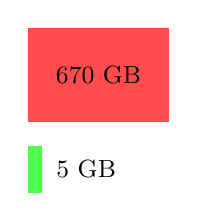
\begin{tikzpicture}[scale=0.6]
\fill[red!70] (0,0) rectangle (3,2);
\node at (1.5,1) {\small 670 GB};
\fill[green!70] (0,-1.5) rectangle (0.3,-0.5);
\node[right] at (0.4,-1) {\small 5 GB};
\end{tikzpicture}
\end{columns}
\end{frame}

\begin{frame}{Video Compression Types}
\begin{columns}
\column{0.5\textwidth}
\begin{block}{Spatial}
Compress individual frames
\end{block}
\begin{block}{Temporal}
Store only changes between frames
\end{block}
\column{0.5\textwidth}
\centering
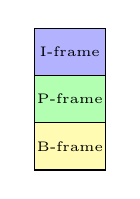
\begin{tikzpicture}[scale=0.6]
\draw[fill=blue!30] (0,2) rectangle (1.5,3);
\node at (0.75,2.5) {\tiny I-frame};
\draw[fill=green!30] (0,1) rectangle (1.5,2);
\node at (0.75,1.5) {\tiny P-frame};
\draw[fill=yellow!30] (0,0) rectangle (1.5,1);
\node at (0.75,0.5) {\tiny B-frame};
\end{tikzpicture}
\end{columns}
\vspace{0.3cm}
\begin{itemize}
\item \textbf{I:} Complete image
\item \textbf{P:} Predicted from previous
\item \textbf{B:} Bi-directional prediction
\end{itemize}
\end{frame}

\begin{frame}{Video Codecs}
\begin{itemize}
\item \textbf{H.264/AVC:} Most widely used, good compression
\item \textbf{H.265/HEVC:} 50\% better than H.264, 4K streaming
\item \textbf{VP9:} Google's codec, YouTube default
\item \textbf{AV1:} Royalty-free, next-gen (Netflix, YouTube)
\item \textbf{ProRes:} Apple's professional codec
\end{itemize}
\begin{exampleblock}{Real Usage}
Netflix uses H.265 for 4K, AV1 for newer content
\end{exampleblock}
\end{frame}

\begin{frame}{Video Container Formats}
\begin{itemize}
\item \textbf{MP4:} Universal, web-friendly (.mp4)
\item \textbf{MKV:} Matroska, supports multiple tracks (.mkv)
\item \textbf{AVI:} Legacy Windows format (.avi)
\item \textbf{MOV:} Apple QuickTime (.mov)
\item \textbf{WebM:} Open format for web (.webm)
\end{itemize}
\begin{alertblock}{Note}
Container $\neq$ Codec. MP4 can contain H.264, H.265, or other codecs
\end{alertblock}
\end{frame}

\begin{frame}{Bitrate and Quality}
\begin{columns}
\column{0.5\textwidth}
\begin{itemize}
\item \textbf{Bitrate:} Data per second
\item Higher = Better quality
\item \textbf{Typical Bitrates:}
\begin{itemize}
\item YouTube 1080p: 8 Mbps
\item Netflix 4K: 25 Mbps
\item Blu-ray: 40 Mbps
\end{itemize}
\item \textbf{CBR:} Constant
\item \textbf{VBR:} Variable
\end{itemize}
\column{0.5\textwidth}
\centering
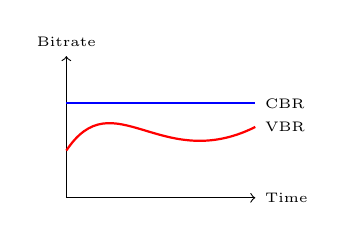
\begin{tikzpicture}[scale=0.6]
\draw[->] (0,0) -- (4,0) node[right] {\tiny Time};
\draw[->] (0,0) -- (0,3) node[above] {\tiny Bitrate};
\draw[thick,blue] (0,2) -- (4,2);
\node[right] at (4,2) {\tiny CBR};
\draw[thick,red] (0,1) .. controls (1,2.5) and (2,0.5) .. (4,1.5);
\node[right] at (4,1.5) {\tiny VBR};
\end{tikzpicture}
\end{columns}
\end{frame}

\begin{frame}{Chroma Subsampling}
\begin{columns}
\column{0.5\textwidth}
\begin{itemize}
\item Reduces color info
\item Keeps brightness
\item \textbf{4:4:4:} Full color
\item \textbf{4:2:2:} Half chroma
\item \textbf{4:2:0:} Quarter chroma
\end{itemize}
\column{0.5\textwidth}
\centering
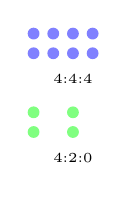
\begin{tikzpicture}[scale=0.5]
\foreach \x in {0,1,2,3}
  \foreach \y in {0,1}
    \fill[blue!50] (\x*0.5,\y*0.5+2) circle (0.15);
\node[below] at (1,1.7) {\tiny 4:4:4};
\foreach \x in {0,2}
  \foreach \y in {0,1}
    \fill[green!50] (\x*0.5,\y*0.5) circle (0.15);
\node[below] at (1,-0.3) {\tiny 4:2:0};
\end{tikzpicture}
\end{columns}
\vspace{0.2cm}
\begin{block}{Why It Works}
Eye more sensitive to brightness than color
\end{block}
\end{frame}

\begin{frame}{Video Streaming Technologies}
\begin{columns}
\column{0.5\textwidth}
\begin{itemize}
\item \textbf{Adaptive Bitrate:} Adjusts to bandwidth
\item \textbf{HLS:} HTTP Live Streaming
\item \textbf{DASH:} Dynamic Adaptive
\end{itemize}
\begin{exampleblock}{Example}
Netflix/YouTube buffer multiple quality versions
\end{exampleblock}
\column{0.5\textwidth}
\centering
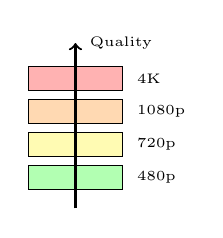
\begin{tikzpicture}[scale=0.6]
\draw[fill=red!30] (0,2.5) rectangle (2,3);
\node[right] at (2.1,2.75) {\tiny 4K};
\draw[fill=orange!30] (0,1.8) rectangle (2,2.3);
\node[right] at (2.1,2.05) {\tiny 1080p};
\draw[fill=yellow!30] (0,1.1) rectangle (2,1.6);
\node[right] at (2.1,1.35) {\tiny 720p};
\draw[fill=green!30] (0,0.4) rectangle (2,0.9);
\node[right] at (2.1,0.65) {\tiny 480p};
\draw[->,thick] (1,0) -- (1,3.5);
\node[right] at (1.1,3.5) {\tiny Quality};
\end{tikzpicture}
\end{columns}
\end{frame}

\begin{frame}{Video Editing Workflow}
\begin{enumerate}
\item \textbf{Capture:} Record or import footage
\item \textbf{Import:} Load into editing software
\item \textbf{Edit:} Cut, trim, arrange clips
\item \textbf{Effects:} Add transitions, color grading
\item \textbf{Audio:} Sync, mix, add music
\item \textbf{Export:} Render final video with codec/format
\end{enumerate}
\end{frame}

\begin{frame}{Summary: Multimedia Basics}
\begin{itemize}
\item Multimedia integrates text, audio, video, graphics
\item Hypermedia adds non-linear navigation
\item WWW is information system on Internet
\item Editing tools: Photoshop, Premiere, Audacity
\item Authoring tools: Unity, Adobe Animate
\end{itemize}
\end{frame}

\begin{frame}{Summary: Graphics \& Color}
\begin{itemize}
\item Raster (pixels) vs Vector (math)
\item JPEG (lossy), PNG (lossless), SVG (scalable)
\item RGB (screens), CMYK (print), HSV (intuitive)
\item Color depth affects quality and file size
\item Color management ensures accurate reproduction
\end{itemize}
\end{frame}

\begin{frame}{Summary: Digital Video}
\begin{itemize}
\item Frame rate: 24-60+ fps
\item Resolution: SD to 8K
\item Compression essential: H.264, H.265, AV1
\item Codecs compress, containers store
\item Streaming uses adaptive bitrate
\end{itemize}
\end{frame}

\begin{frame}{References \& Further Learning}
\begin{itemize}
\item \textbf{Books:}
\begin{itemize}
\item "Fundamentals of Multimedia" by Ze-Nian Li
\item "Digital Video and HD" by Charles Poynton
\end{itemize}
\item \textbf{Online Resources:}
\begin{itemize}
\item MDN Web Docs (color models)
\item FFmpeg documentation (video processing)
\item Adobe tutorials (editing tools)
\end{itemize}
\end{itemize}
\end{frame}

\begin{frame}
\centering
\Huge Thank You!\\
\vspace{1cm}
\Large Questions?
\end{frame}

\end{document}
